\section{Desenvolvimento}

\subsection*{Parte 1}

Foram recolhidos dados de amostra para os movimentos de vibração nos eixos X, Y e Z, movimento circular no eixo Z e movimento de rotação em torno de um ponto fora do objeto no eixo Y.

Nas figuras abaixo vemos os dados recolhidos. Em cada imagem temos 6 gráficos referentes respectivamente à aceleração 3 eixos e giroscópio nos 3 eixos.
Podemos também ver que tivemos etapas de resolução do movimento e etapas de repouso.


\begin{figure}[H]
    \center
    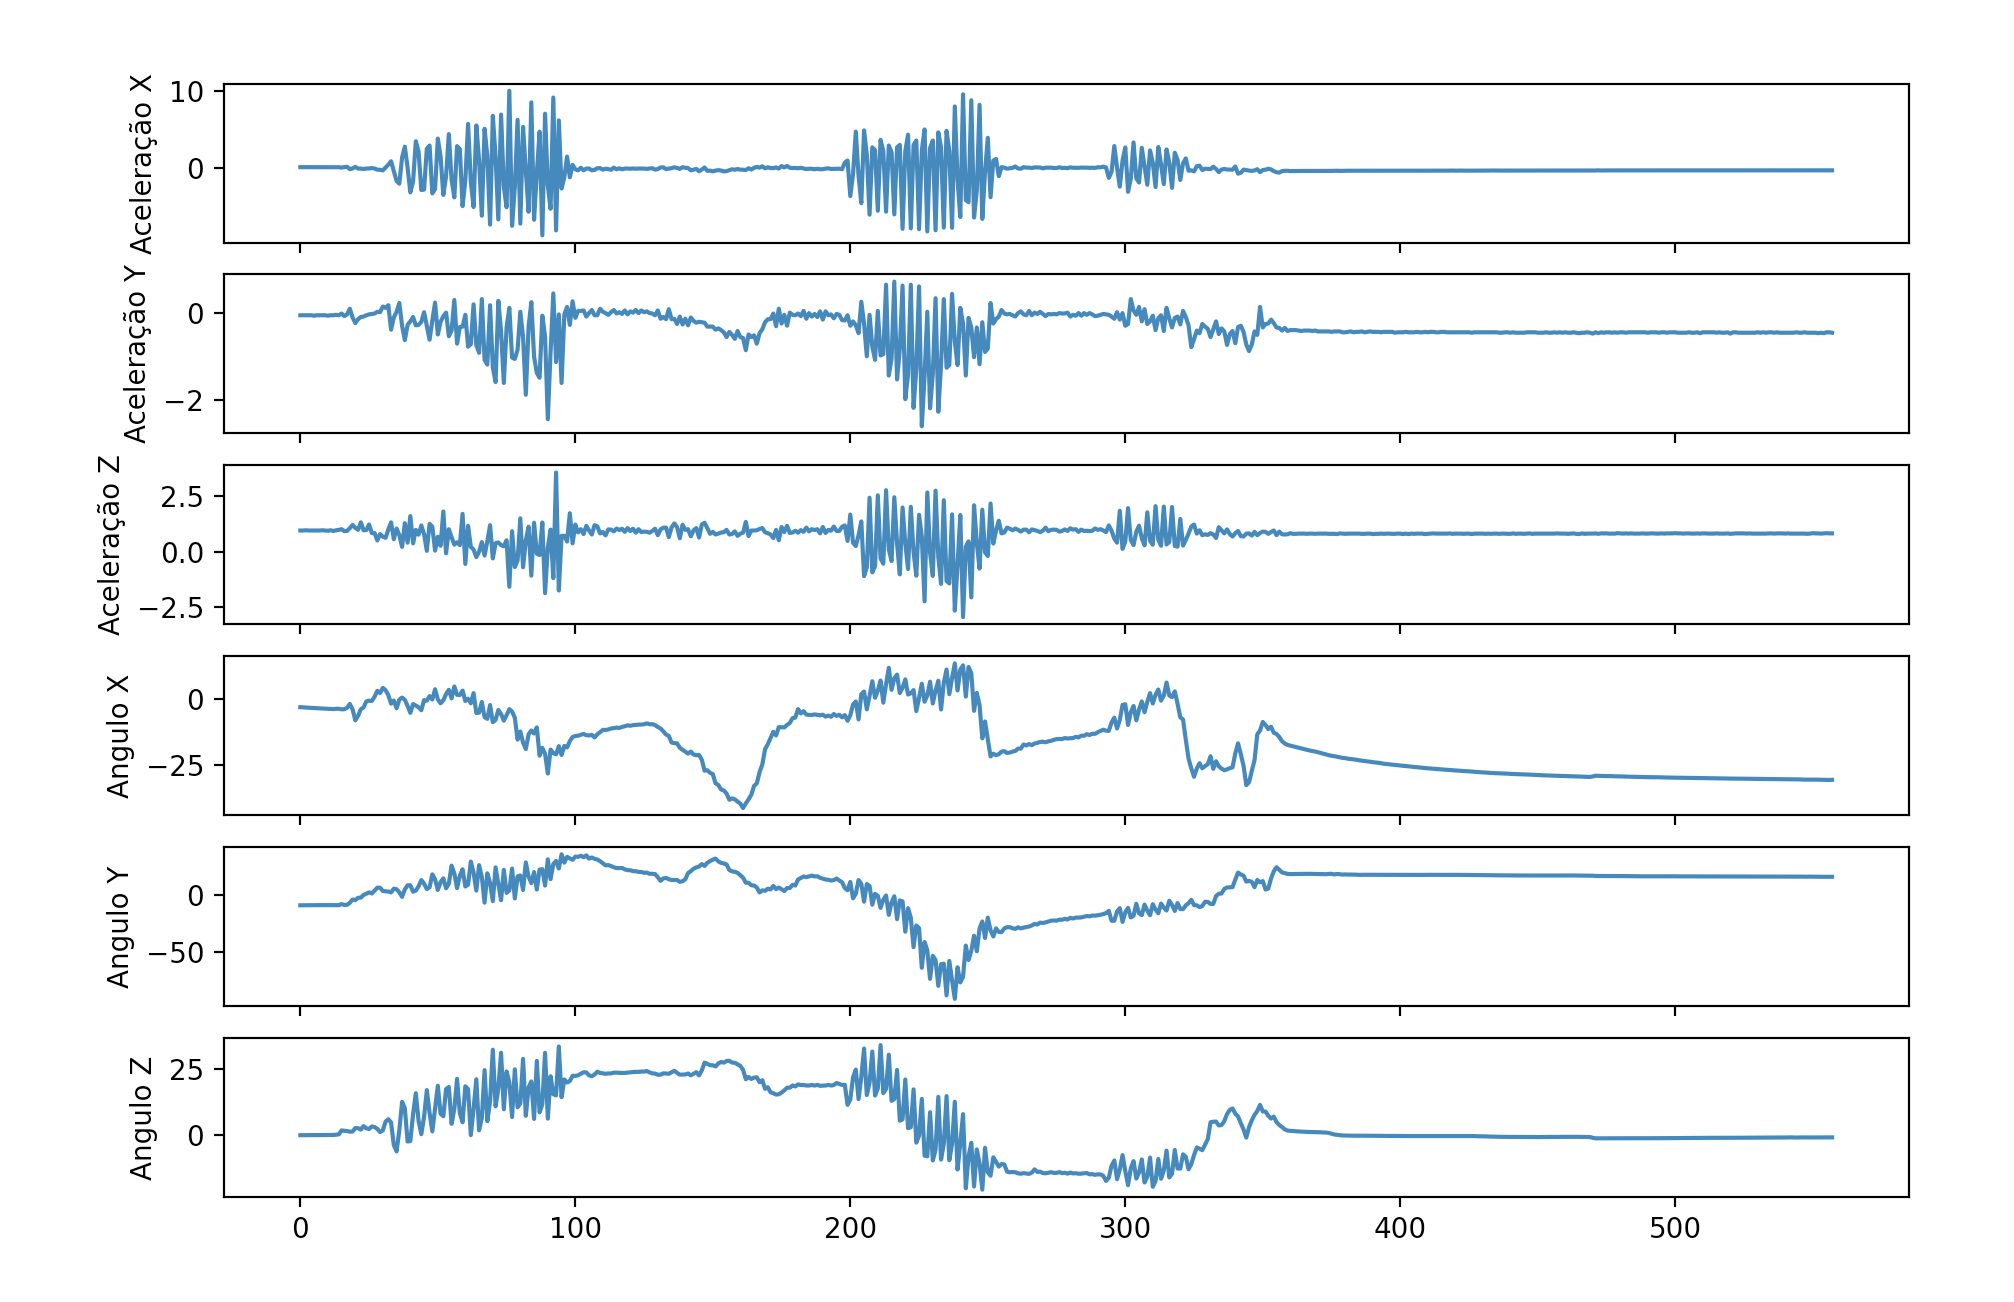
\includegraphics[width=7cm]{images/VibracaoX.png}
    \label{img6}
    \caption{Vibração no eixo X}
\end{figure}

\begin{figure}[H]
    \center
    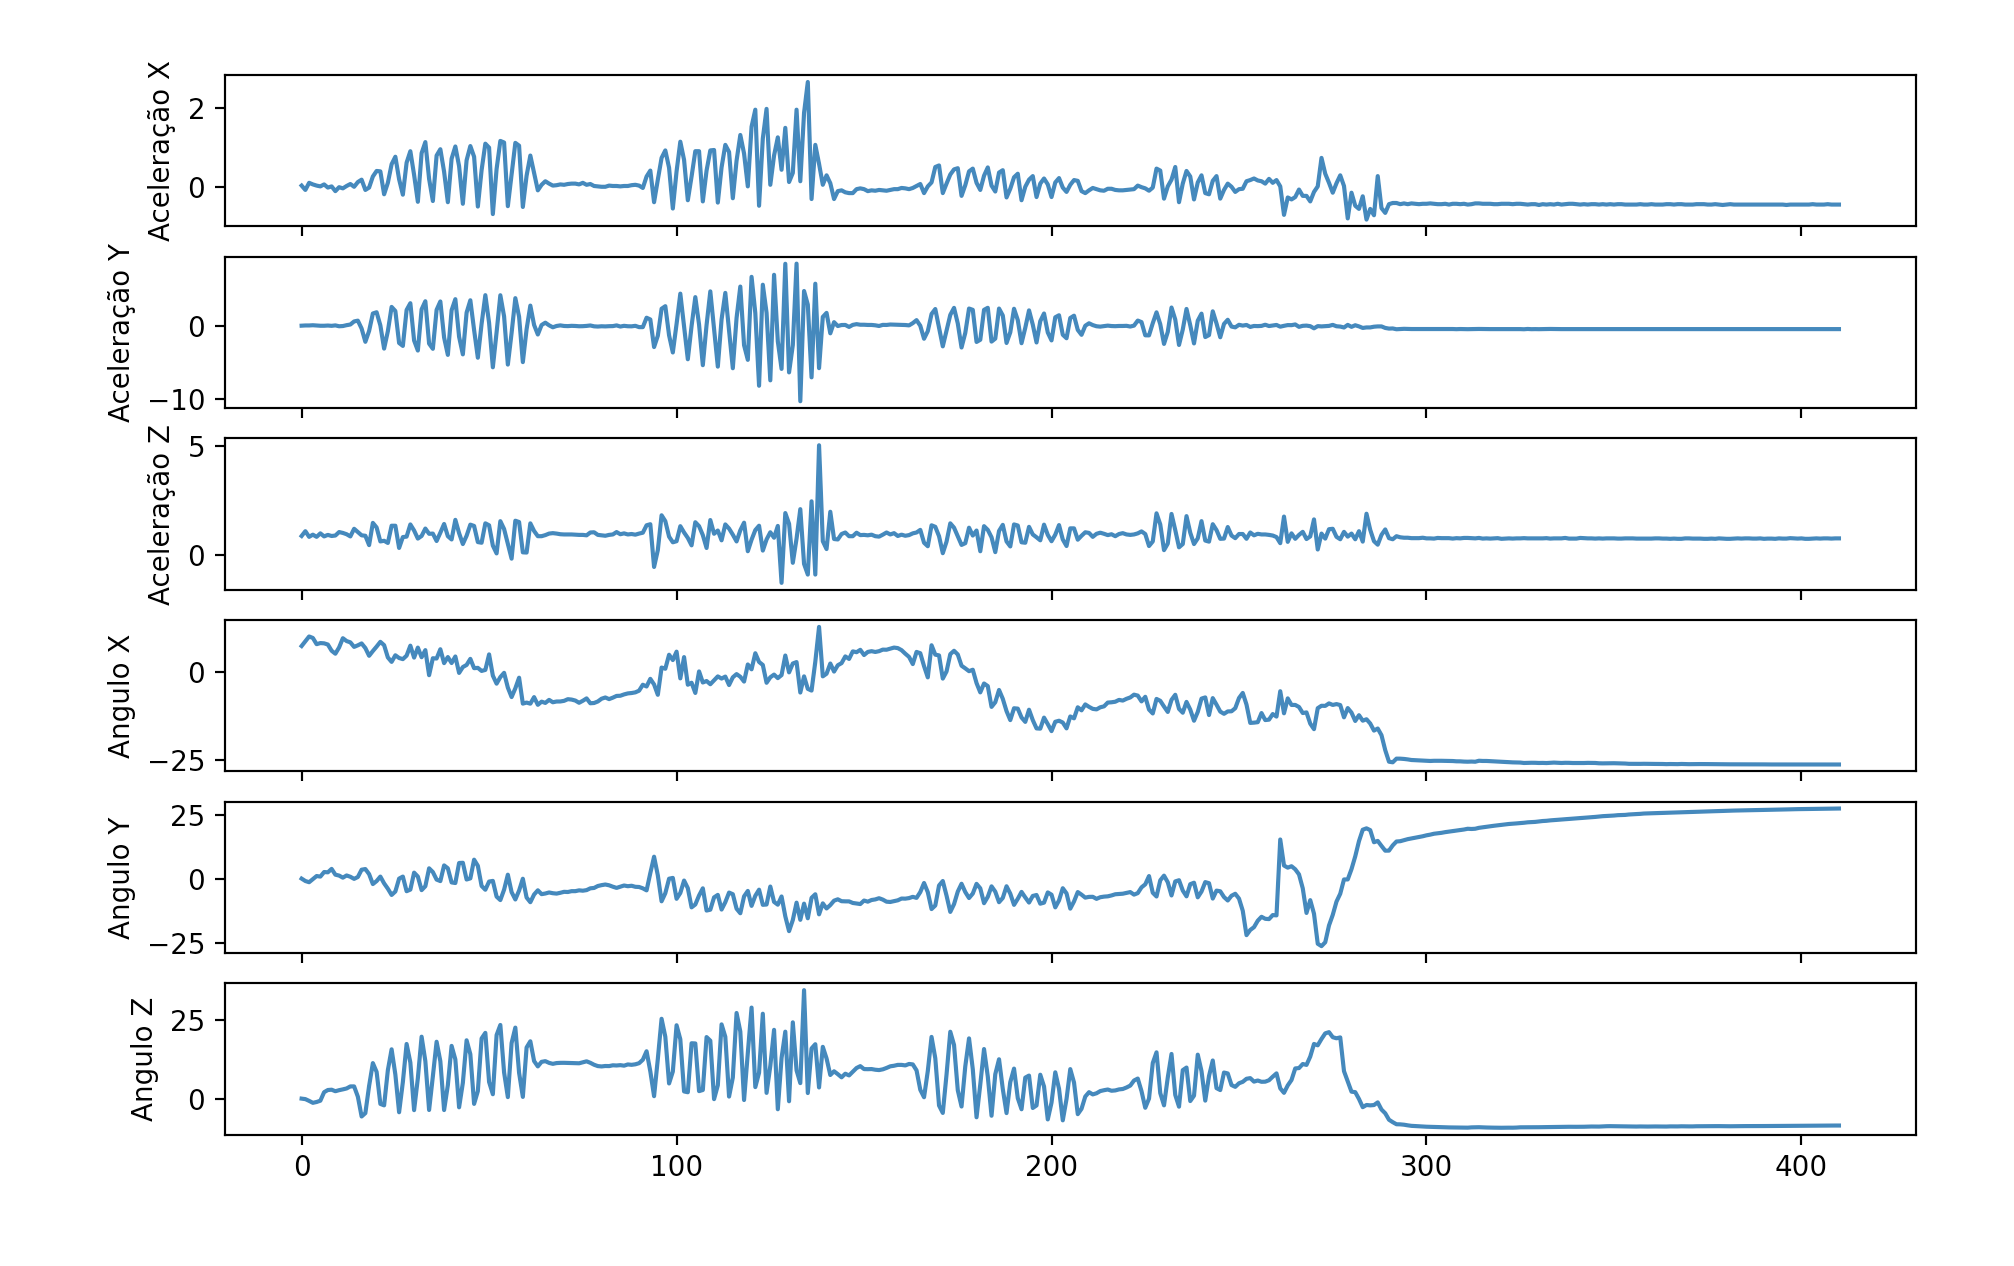
\includegraphics[width=7cm]{images/VibracaoY.png}
    \label{img2}
    \caption{Vibração no eixo Y}
\end{figure}

\begin{figure}[H]
    \center
    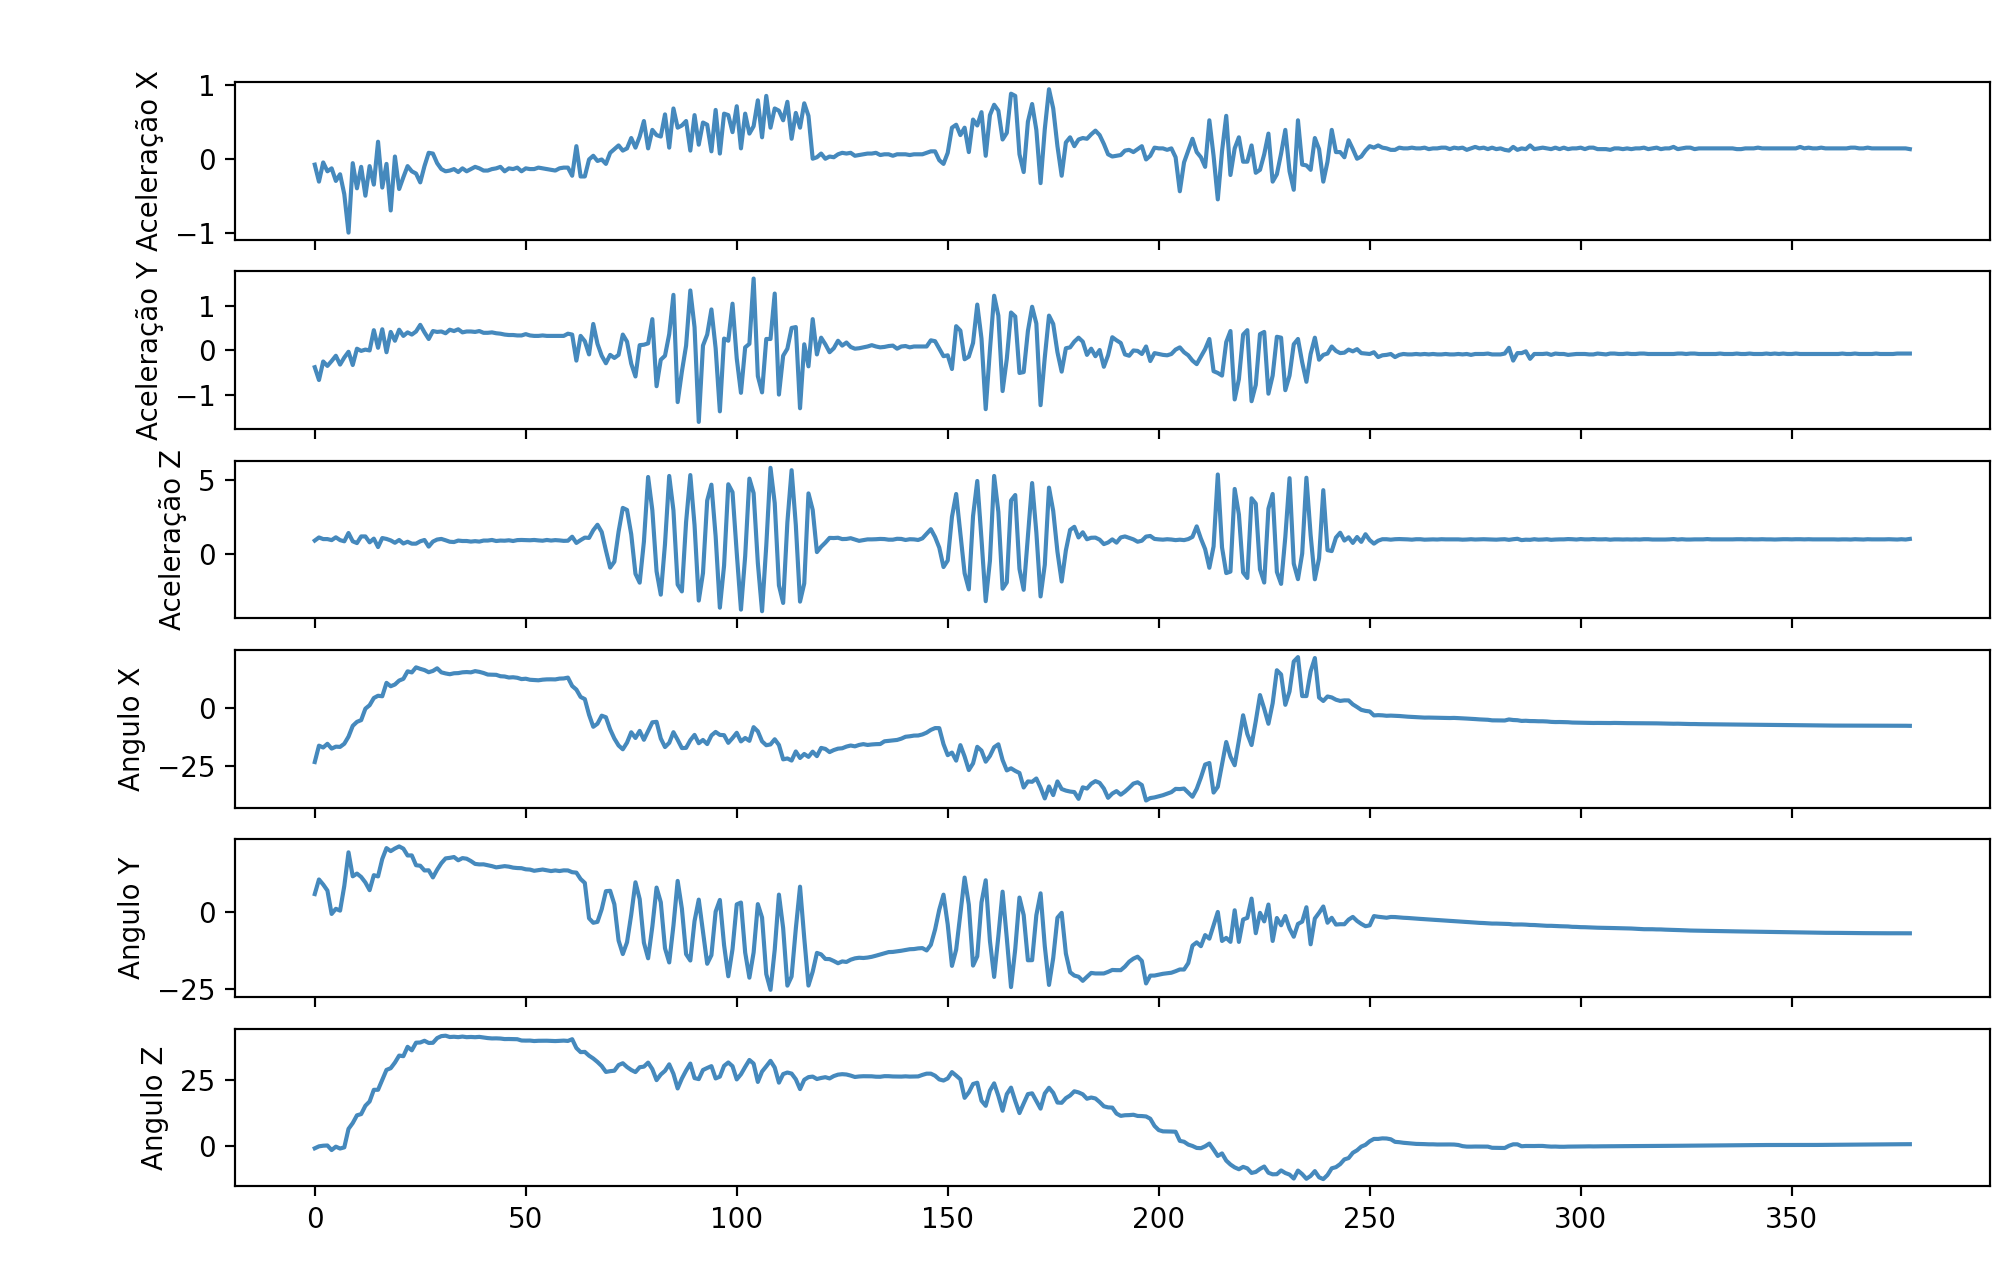
\includegraphics[width=7cm]{images/VibracaoZ.png}
    \label{img3}
    \caption{Vibração no eixo Z}
\end{figure}

\begin{figure}[H]
    \center
    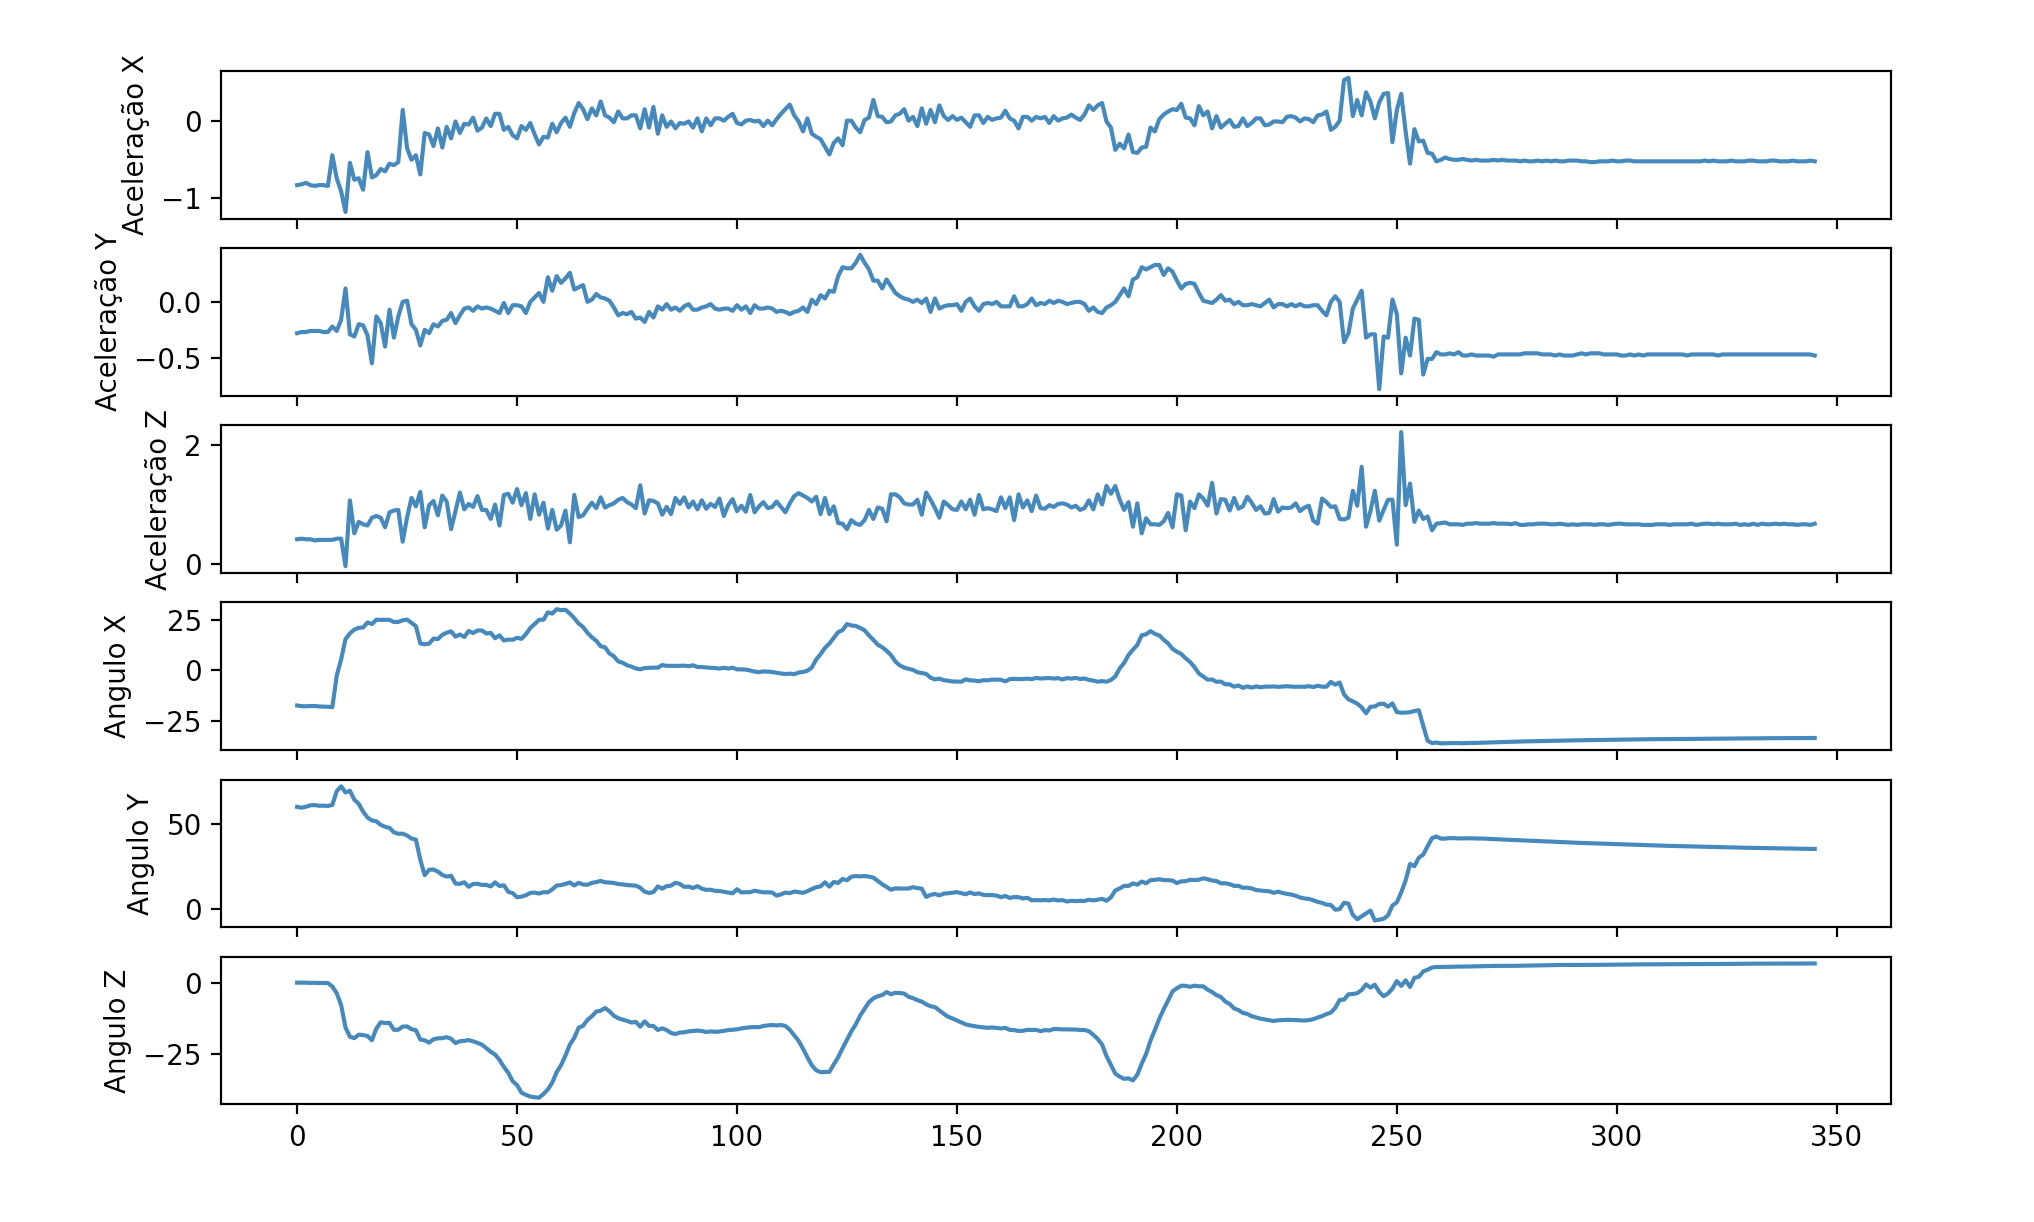
\includegraphics[width=9cm]{images/CirculoZ.png}
    \label{img4}
    \caption{Movimento circular no eixo Z}
\end{figure}

\begin{figure}[H]
    \center
    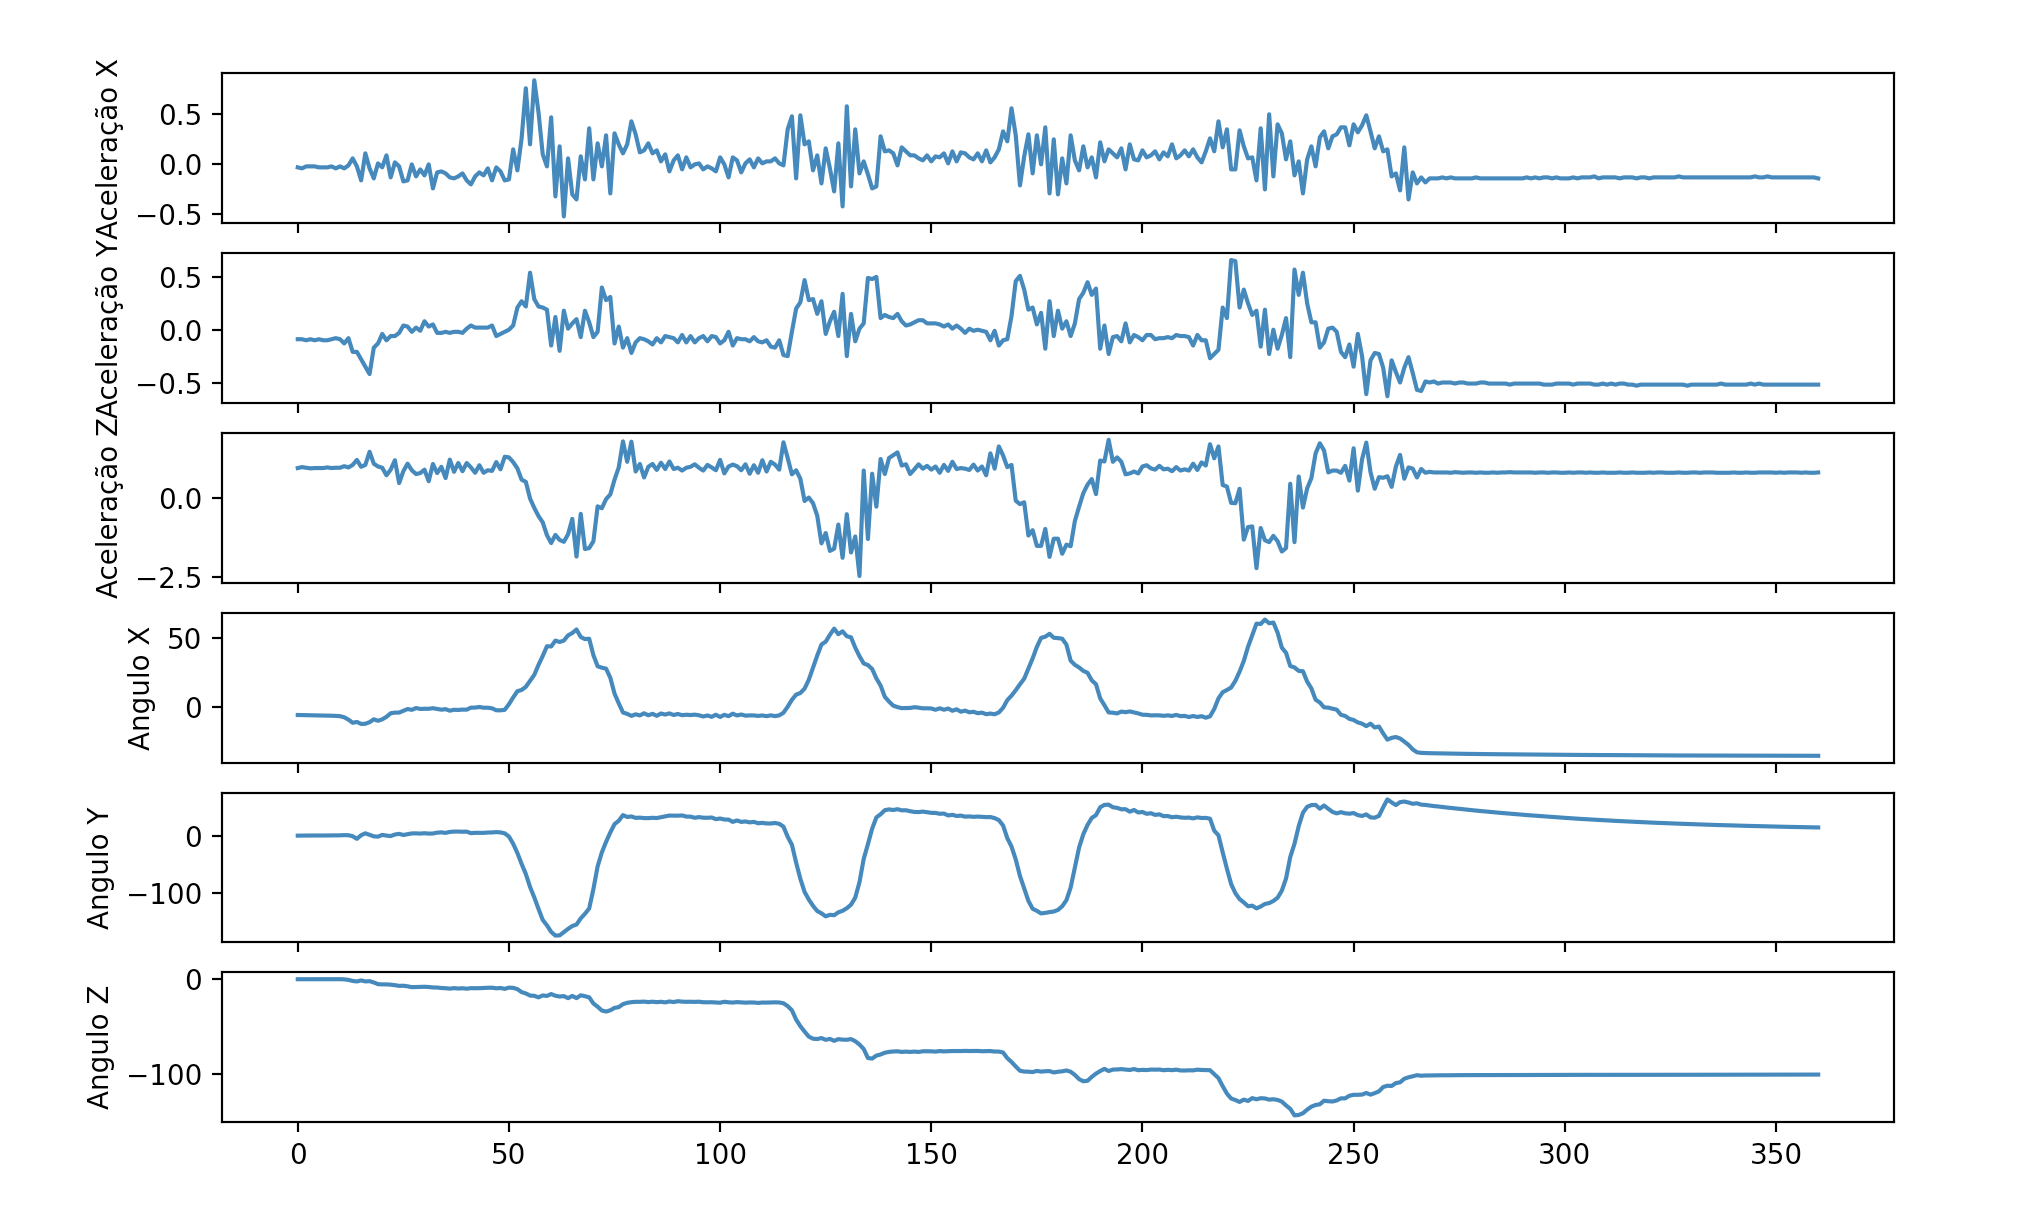
\includegraphics[width=9cm]{images/GiraeVoltaY.png}
    \label{img5}
    \caption{ Movimento de rotação 180 graus no eixo Y, ida e volta }
\end{figure}


\subsection*{Parte 2}

Utilizando site \hyperlink{https://towardsdatascience.com/feature-engineering-on-time-series-data-transforming-signal-data-of-a-smartphone-accelerometer-for-72cbe34b8a60}{towardsdatascience}
como auxílio para feature engineering com dados de acelerômetro, extraí um código em python capaz de calcular:


1. mean

2. standard deviation

3. average absolute deviation

4. minimum value

5. maximum value

6. difference of maximum and minimum values

7. median

8. median absolute deviation

9. interquartile range

10. negative values count

11. positive values count

12. number of values above mean

13. number of peaks

14. skewness

15. kurtosis

16. energy

17. average resultant acceleration

18. signal magnitude area


Desses irei fazer uma analise com os dados:
Usarei apenas mean, median, number of peaks, energy, signal magnitude area, avg resultant


\subsection*{Parte 3}


Antes de definir os valores estatíisticos de cada tipo de movimento é preciso separar cada janela de dados correspondente ao inicio e fim do movimento.
Nas figuras 7 e 8 podemos ver os dados de 1 amostra de vibração X e seus respectivos valores estatísticos.


\begin{figure}[H]
    \center
    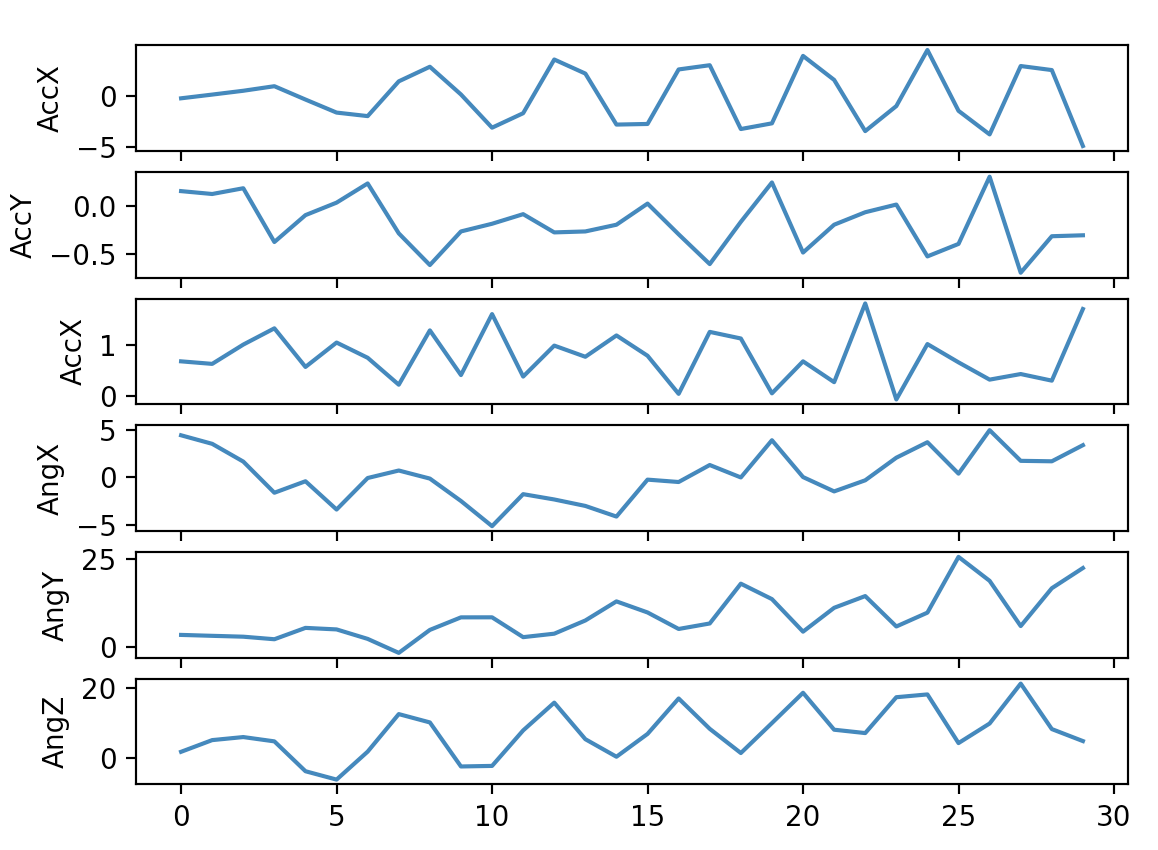
\includegraphics[width=9cm]{images/VibracaoX_1_raw.png}
    \caption{Amostra de Vibração no eixo X}
\end{figure}

\begin{figure}[H]
    \center
    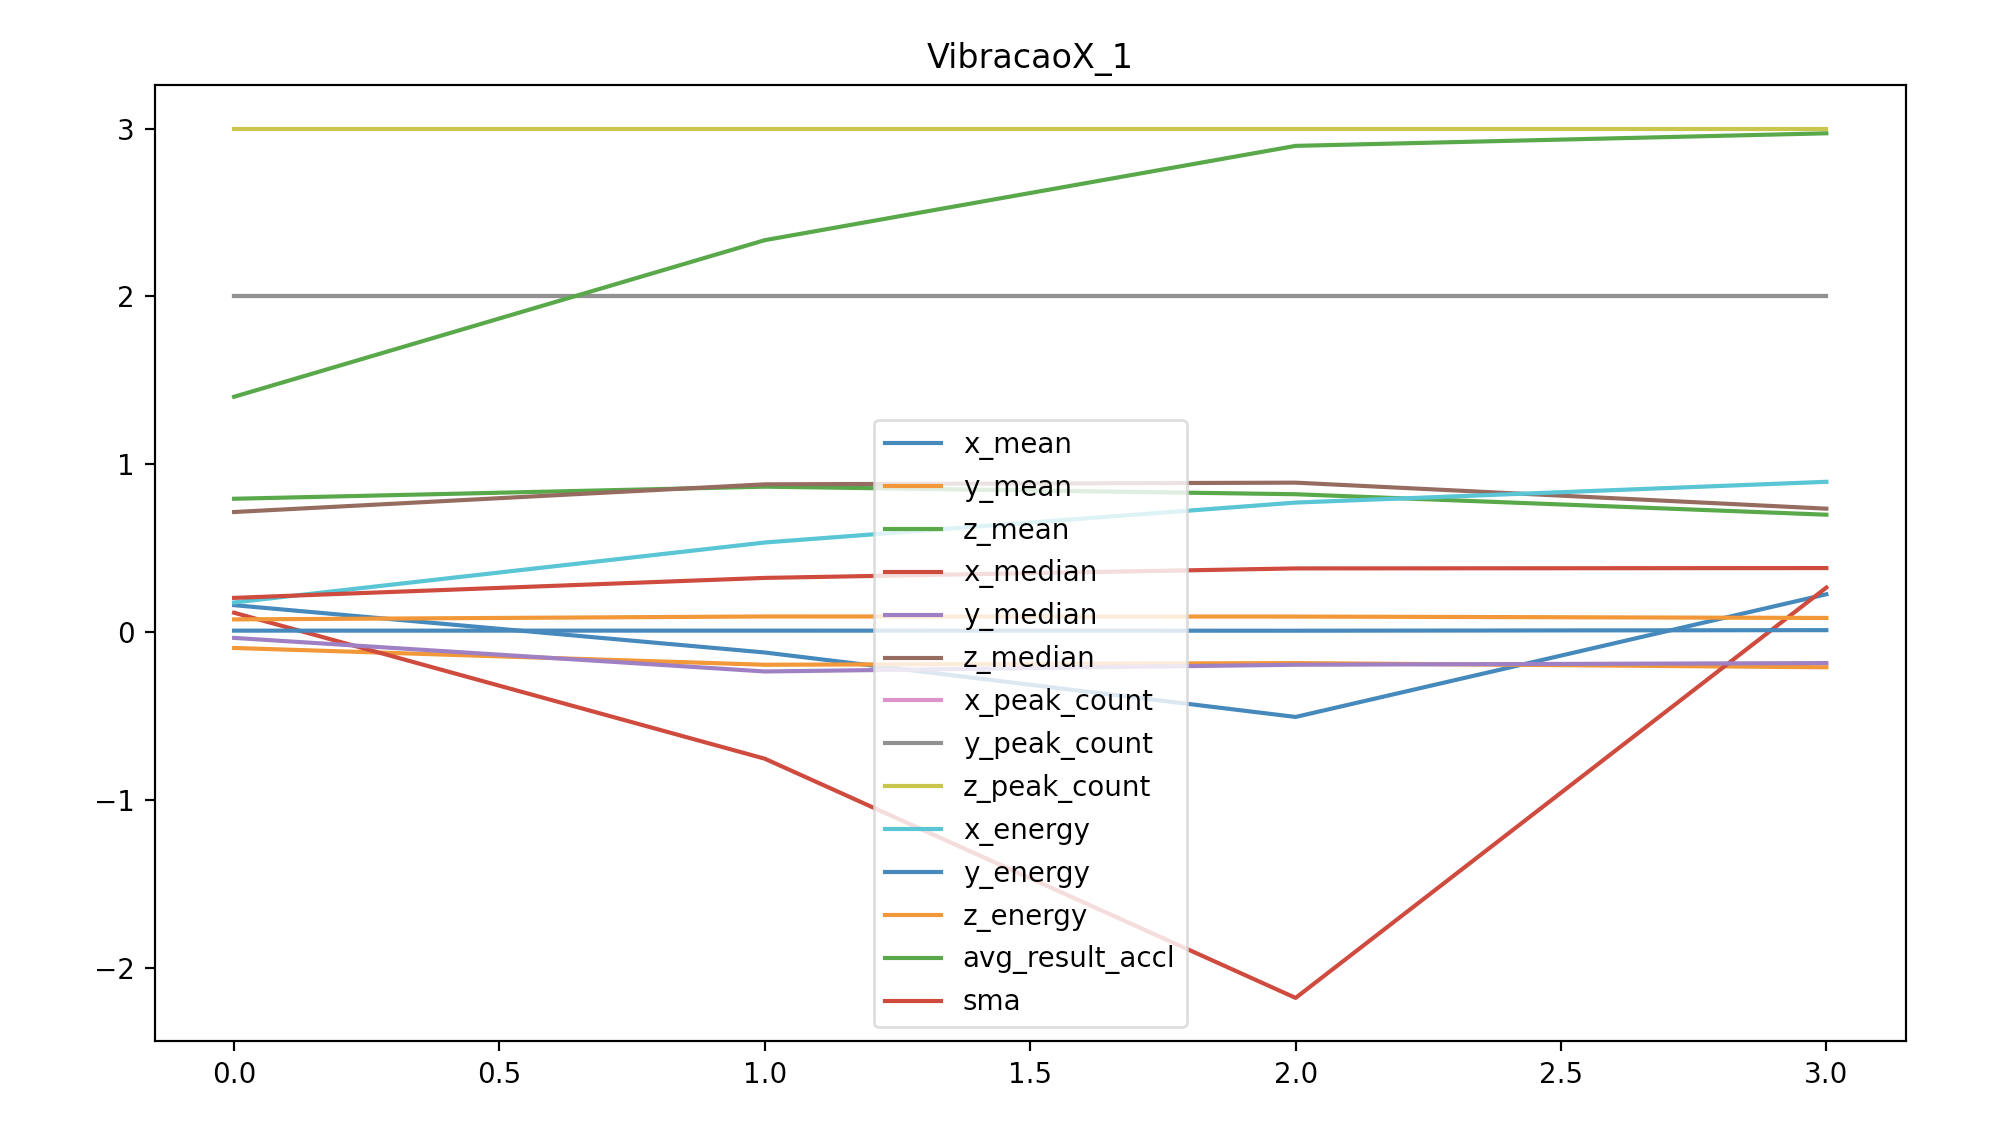
\includegraphics[width=9cm]{images/VibracaoX_1_stats.png}
    \caption{ Valores abstraídos da amostra de vibração em X }
\end{figure}


Abaixo temos a mesma representação porém com o objeto no estado Parado.


\begin{figure}[H]
    \center
    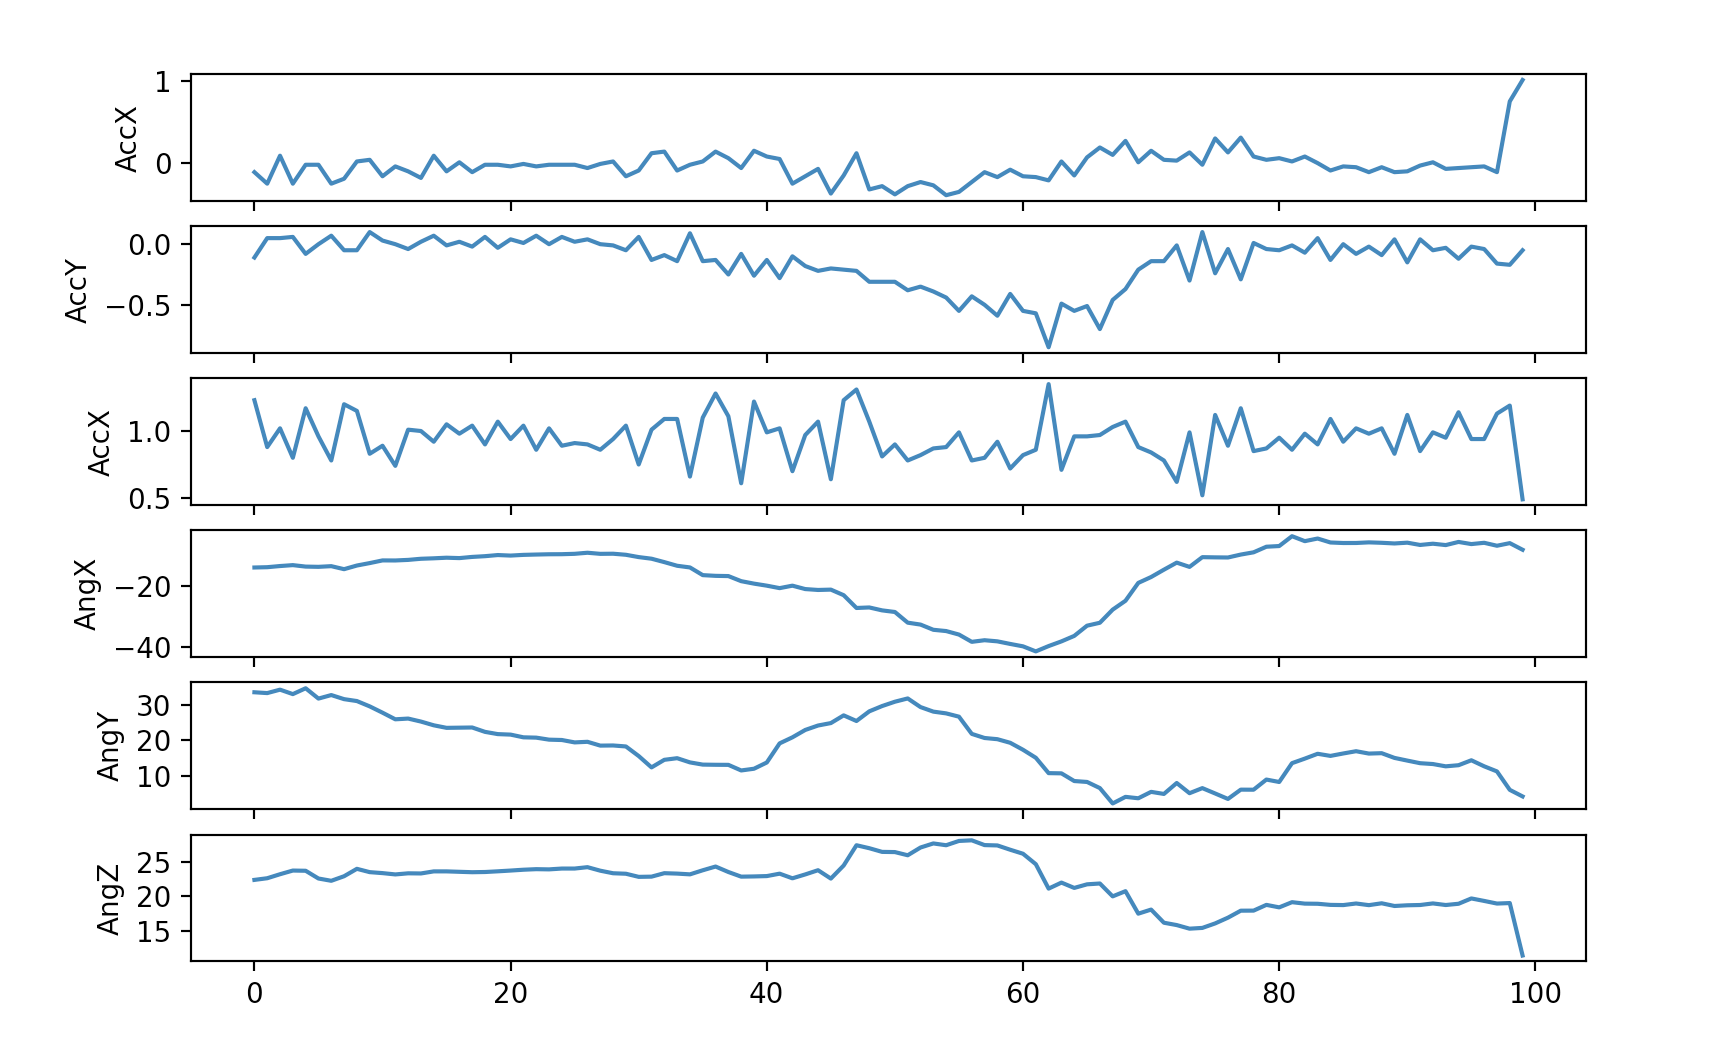
\includegraphics[width=9cm]{images/Parado_1_raw.png}
    \caption{Amostra de objeto Parado}
\end{figure}

\begin{figure}[H]
    \center
    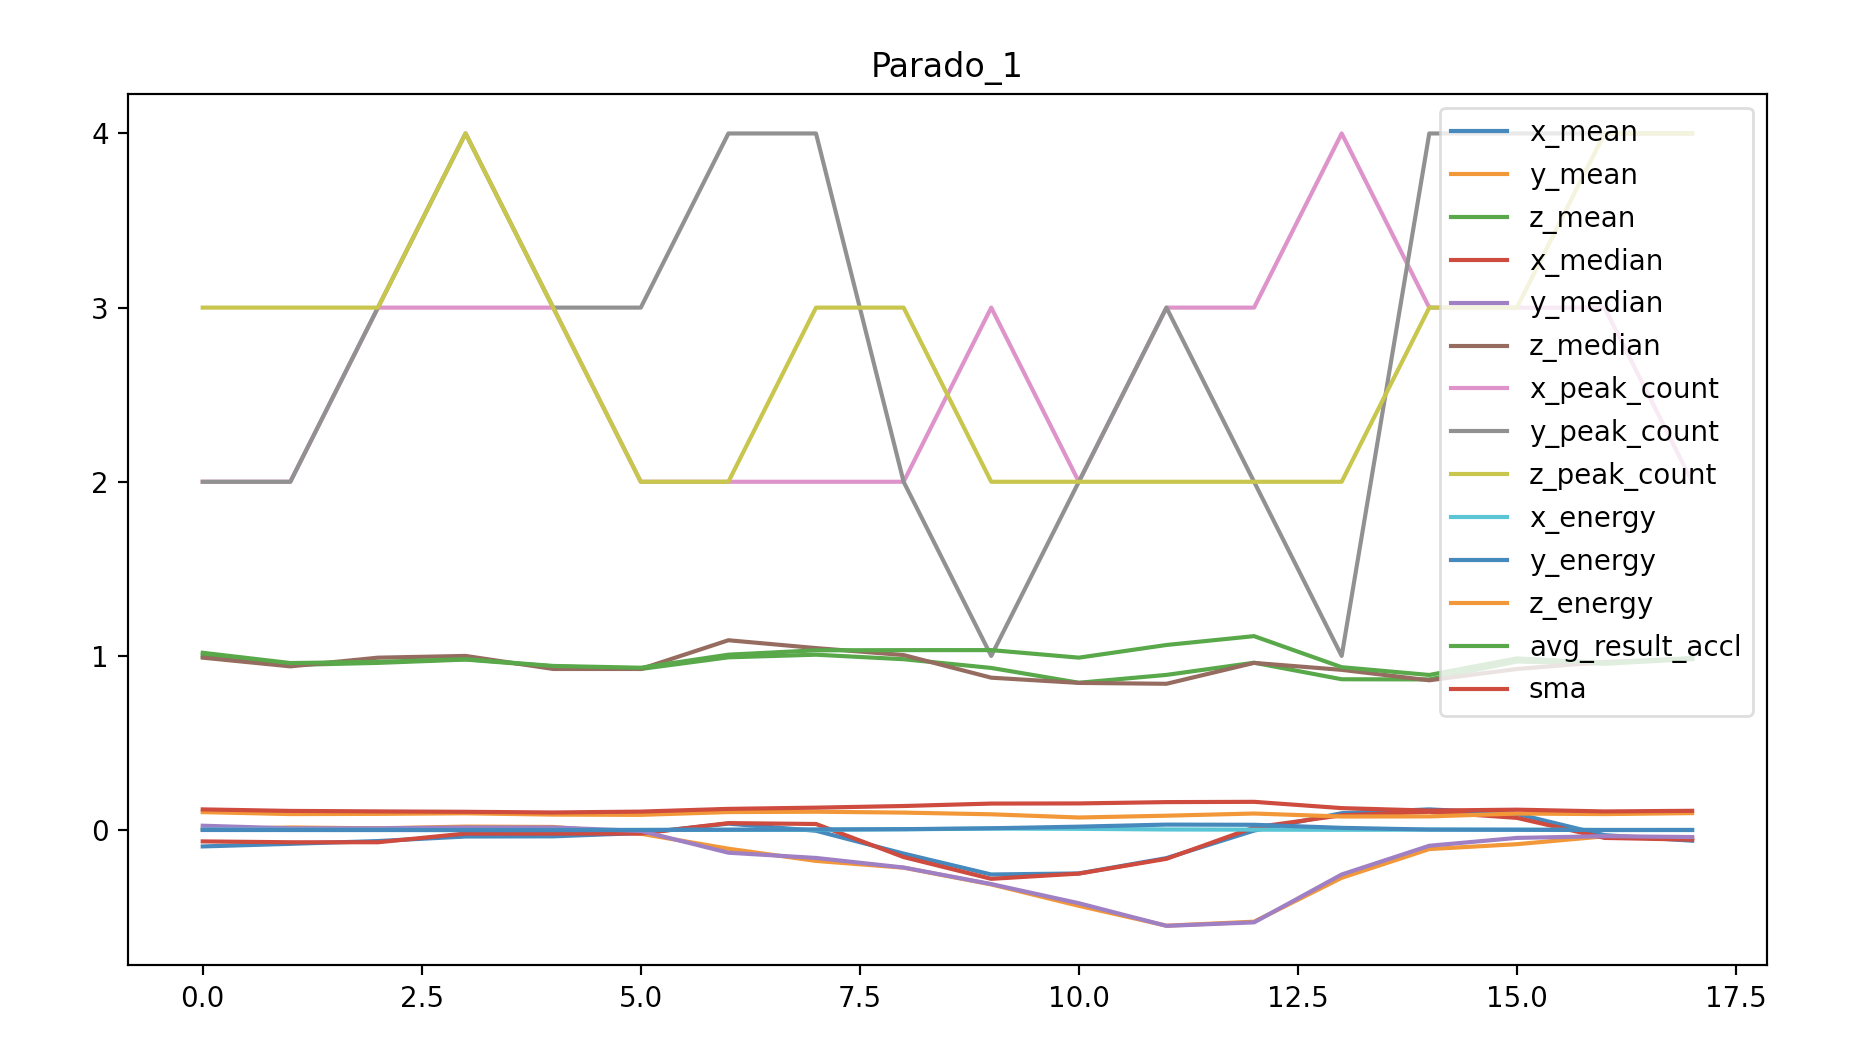
\includegraphics[width=9cm]{images/Parado_1_stats.png}
    \caption{ Valores abstraídos da amostra de Objeto parado }
\end{figure}

